%caseBldg

1. Single zone building model from ...

2. Specification for comfort when occupied.

3. 24 hour look ahead, given disturbances and occupancy. Initial guess (with negative robustness) via solving an LP.

4. Can be applied in a receding horizon manner. For the given setting, could very well be solved using a linear program asking for temperature between 22-28C for time steps 10 to 19, but we use our method to illustrate how robustness based control can be used to satisfy a specification. The next example (Autonomous ATC) shows control with a specification cannot be trivially translated to a linear program with Polyhedral constraints.

5. Figure shows room temperature for the 3 methods (other states and disturbances/control in a single figure if necessary)

6. Table shows robustness of obtained trajectory via the 3 methods. Note, Optimal solution would be temperature of 25C  (robustness of 3) for the occupancy period (if dynamics/constraints would allow it).

\begin{figure}[t]
\centering
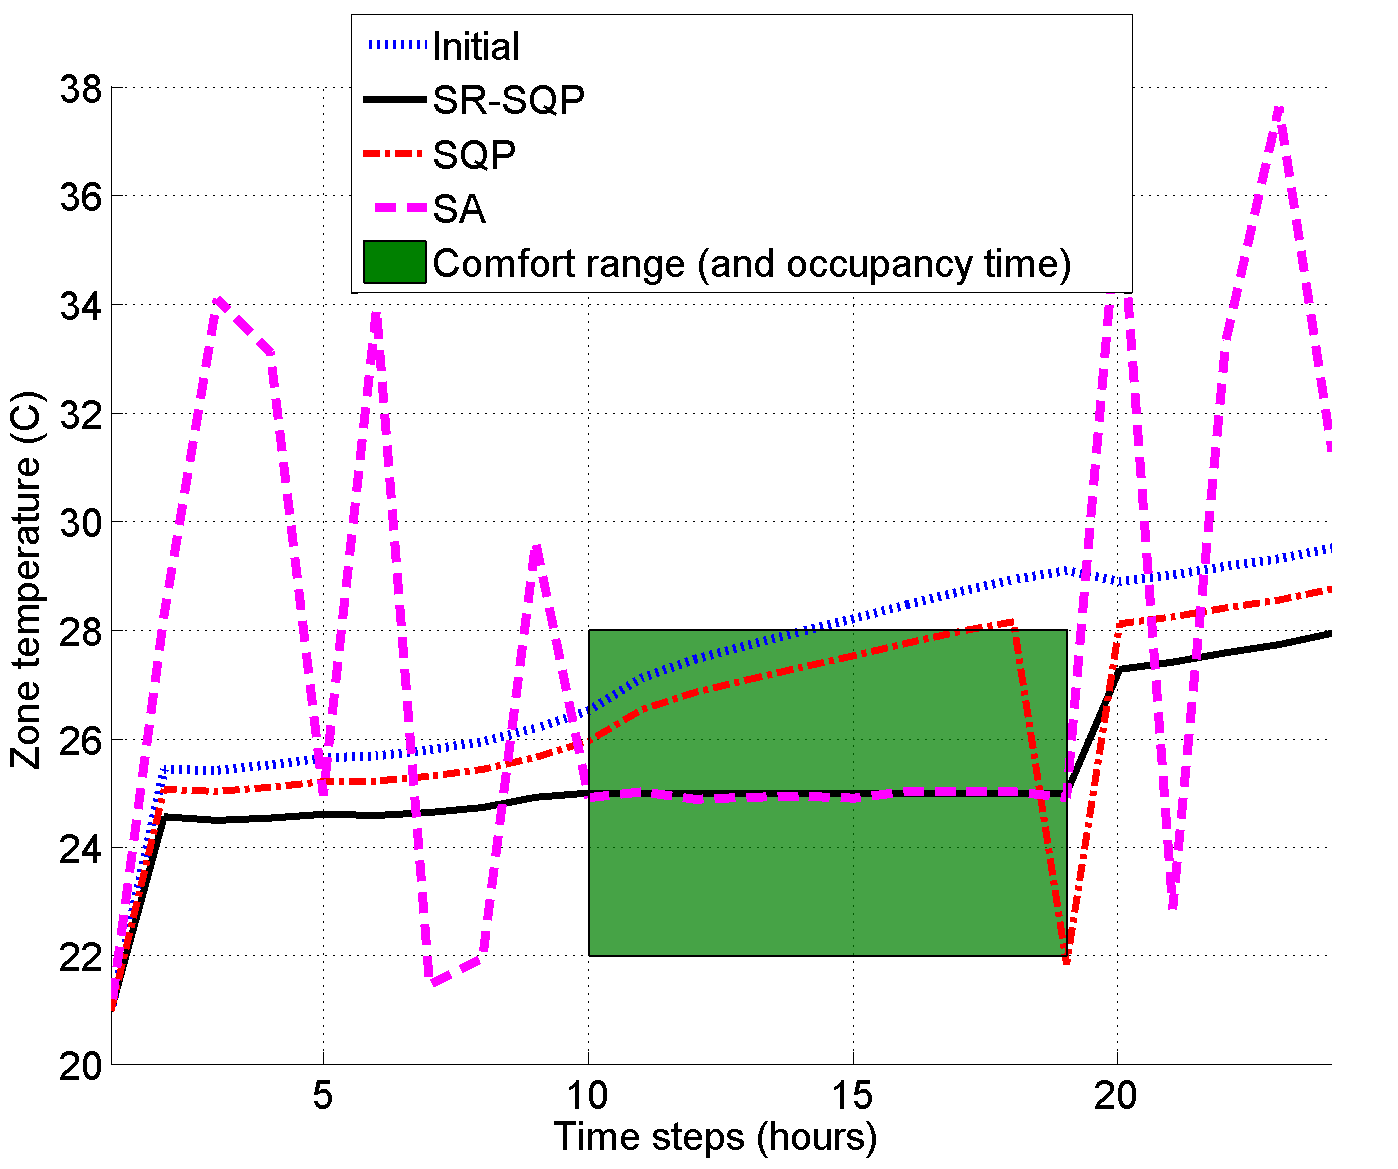
\includegraphics[width=0.49\textwidth]{figures/ZoneTemp_scissored}
\caption{Zone temperatures. The green rectangle shows the comfortable temperature limit of 22-28 C, applicable during time steps 10-19 (when the building is occupied, 9am-6pm).}
\label{fig:ZoneTemp}
\end{figure}
